\chapter{Introduction}

The advancement of technology has opened new avenues for innovation in construction.
The use of robots in the assembly of timber structures presents a new frontier in this field.
This interdisciplinary PhD thesis focuses on the integration of industrial robots and distributed robotic tools (DiRT) for the automatic assembly of timber structures.
Specifically, timber frame structures with integral timber joints. 

Despite the potential benefits that automation could bring to the construction industry, the necessary technology to achieve this goal remains unknown. The objective of this thesis is to embark on a journey of discovery and innovation that will contribute to the advancement of knowledge in the field.
By combining interdisciplinary approaches from timber construction, computational design and robotics, this research will provide insights into the technical and operational aspects of the automatic assembly process, as well as its potential benefits and challenges.
Through the development of novel solutions and empirical construction experiments, this PhD thesis aspires to shape the future of construction and contribute to the interdisciplinary field of digital fabrication, between architecture, construction and robotics.

\section{Timber Frame Construction}
\label{sec:timberframeconstruction}
Timber construction has been used historically in many cultures with an ample supply of trees.
Timber is a remarkable construction material because of its very high strength-to-weight ratio.
It can withstand tension and compression, making it suitable for different structural roles. Moreover, timber can naturally reach lengths of many metres, which provides tall columns and long beams for the construction of architectural structures at various scales.
Historically, many types of construction methods have been developed. The focus of this thesis is timber frame construction which refers to a range of timber construction methods used as early as the 12th century until the early 20th century \parencite{sobonTimberFrameConstruction1984}.

\subsection{Defining Characteristics}
\label{subsec:timberframeconstruction/definingcharacteristics}

We can understand timber frame construction as a set of techniques that have evolved over time. Carpenters have experimented with different joint designs, structural arrangements and methods to frame walls, floors and roofs. While these techniques evolved independently in different civilisations, similar material behaviour (e.g. anisotropicity of wood, prone to decay) and similar design goals (e.g. weather protection) resulted in many similarities between them \parencite{zwergerWoodWoodJoints2012}.
While there are still differences between regional practices (caused by regional timber species, weather, local culture and ornamental preferences), the type of timber construction that dominated the pre-industrial era (especially in Europe, North America, and Japan) share similar defining characteristics: (1) Large timber sizes, (2) integral timber joints, and (3) post-and-beam framing. 
These characteristics make timber frame construction ideal for studying automatic assembly.
As such, this thesis is not referring to the timber frame construction of a specific location or time period, but rather to the general use of these three defining characteristics of timber frame construction.

\subsubsection{Large Timber Size}
\label{subsec:timberframeconstruction/largetimbersize}

The first defining characteristic of timber frame construction is large timber sizes.
Historically, this is the result of using a whole harvested tree trunk as a structural member instead of laboriously cutting them into smaller pieces.
It was only after the industrialisation of sawmills that timber could be efficiently cut into smaller dimensions.
Around the same time, the depletion of large trees in Europe and America prompted the more contemporary invention of stick framing construction (i.e. balloon framing and platform framing) that uses dimensional lumber (e.g. 2x4 inch “two-by-four” studs). Later as timber glue technology improved, the use of glue-laminated timber (glulam), laminated veneer lumber (LVL) and other engineered timber products began to appear and allowed the manufacturing and use of large timber elements again.
In this thesis, the assembly of both solid timber and engineered timber is investigated.
The nominal size being used is 100mm x 100mm square profile (see 4.1.3 Scope for Initial Development Round)

\subsubsection{Integral Timber Joints}
\label{subsec:timberframeconstruction/integraltimberjoints}

The second defining characteristic in timber frame construction is the use of integral timber joints (ITJ), where the jointing geometry is carved into the material. Structural load is transmitted from element to element directly through contact pressure over the mating surfaces of the joint. The design of these joints has been refined empirically throughout history, converging into specialised designs according to which structural elements they are connecting \autocite{jacksobonHistoricAmericanTimber2014}. It is common for a joint to serve multiple purposes and thus withstands different types of loads, such as self-weight and live forces. Different ‘geometrical features’ can therefore be incorporated into the connection to meet different force conditions. For example, a lap joint for a floor joist can be combined with a dovetail feature to provide tension resistance.
These joints are typically dry-fitted \footnote{because historical glue technology could not withstand structural forces} and held in place due to interlocking geometry and gravity.
Additionally, it is possible to include metal components in integral timber joints.
This is more common in contemporary design, where metal screws, dowels and tie rods are used to improve joint capacity or to reduce the need to cut complicated joinery.
For the purpose of studying automatic assembly, integral timber joints provide a unique advantage because they can be prefabricated with high accuracy (see 1.1.2.1 Automatic machining of parametric timber joints) and are quick to install.
In this thesis, the assembly of dry-fitted joints both with and without fasteners is explored.
As of today, there is no single consensus in the nomenclature of timber joints as different cultures have historically named their joints using different methods \parencite{satoCompleteJapaneseJoinery1995,seikeArtJapaneseJoinery1977a,sumiyoshiWoodJointsClassical1991}. The first naming convention (commonly used in American and European traditions) is based on the location of the joint and the structural elements it connects to, for example, ‘floor joist joint’ or ‘tying joint below plate’. The second naming convention is based on the joint's geometrical features, for example, ‘dovetail joint’ or ‘scarf lap joint’. Some unique joint designs could also be named according to the use in a famous building. For example, Osaka-jo-otemon-hikae-bashira-tsugite refers to Osaka Castle-Otemon Gate's pillar splice. For the purpose of studying assembly problems, this thesis proposes the use of a different convention that is based on the assembly direction related to the joint (see Section 4.2.1 Lap Joint Classification by Assembly Direction).
The photo below shows timber frame components being assembled on the ground. Notice the use of large timber sizes and integral timber joints. 

(Credits: CC AS 4.0 Licence photo by Georg Hefter - Traditionelles Fachwerk und Timberframe im Vergleich auf georghefter.de)

\subsubsection{Post and Beam Structure}
\label{subsec:timberframeconstruction/postandbeamstructure}

The third defining characteristic of timber frame construction is post-and-beam structural framing \parencite{jacksobonHistoricAmericanTimber2014,sobonTimberFrameConstruction1984}. The use of large timber sizes in timber frame structures allows them to be strong enough without the use of continuous load-bearing walls. The main benefit is the flexible arrangement of floors and walls to suit different architectural programmes. 
On the other hand, integral timber joints are generally weak in rotational stiffness, causing the joints to behave kinematically. Therefore, diagonal bracing is often introduced to fully or partially triangulate the structure to improve structural stiffness. Being limited by the joint design, these bracings function primarily in compression. It is, therefore, common to design the bracings in complementary pairs to resist dynamic wind loads coming from opposing directions. While some architectural designs may find the intrusion of diagonal bracings obtrusive to usable space, these diagonal bracings are highlighted on the facade as ornamentation in half timber designs \parencite{gernerFachwerkEntwicklungGefuege1979}. In this thesis, the demonstration structures are designed with similar structural principles, specifically the use of structural triangulation in the design offered unique stability advantages during the robotic construction process (see 7.1.1 Deformation-Awareness and Error Correction by Triangulation and 7.5.2.6 Global Correction Approach).

The image below shows an example of a half-timber style timber frame house in Soest, Germany. Notice the exposed diagonal elements on the facade.

\begin{figure}[h]
    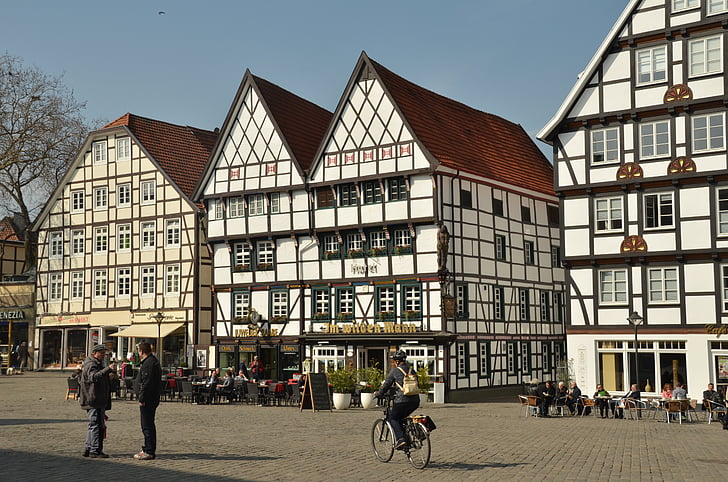
\includegraphics[width=1.0\textwidth]{
        ./auto_convert/Chapter 1 to 3/images/image9.jpg}
    \caption{
        Credits: Licence-free photo, retrieved from \url{https://www.hippopx.com/en/germany-soest-architecture-timber-framed-half-timbered-house-square-city-402214} , n.d.}
\end{figure}
    
\subsection{Current Practice of Timber Frame Construction}

Timber frame construction was once the dominant building method, but it gradually declined in popularity during the 19th and 20th centuries. The advent of industrialization and mass production led to the availability of cheaper building materials such as steel and concrete, which were faster and easier to use. Even within the timber construction sector, newer construction methods that use dimensioned lumber, glulam, LVL, and cross laminated timber (CLT) have replaced timber frame construction. However, in recent years, as more people are aware of the environmental benefits of wood construction, interest in timber frame construction is increasing again as an alternative way to construct with timber. 

Advancements in engineering and design, as well as increased availability of sustainably sourced timber, have helped to make timber frame construction a more viable option for modern building projects. Timber frame components can be prefabricated off-site, which can reduce construction time and costs while also minimising waste and environmental impact. The use of dry-fitted integral timber joints reduces the number of fasteners and components involved, meaning less metal consumption and quicker installation on-site. Finally, timber frame structures can be aesthetically pleasing as they often expose the beautiful timber material and reveal the structural load paths. When the joint details are exposed, they can evoke a feeling of tradition and craftsmanship and are often well-appreciated by those who inhabit the building.

\subsubsection{Automatic Machining of Timber Joints}

Between the years of decline and its recent resurgence, a number of technological improvements have made timber frame construction more efficient and competitive. One of the major advancements has been the use of automatic joinery machines for carving integral timber joints. Traditionally crafted with hand tools, these joints were labour-intensive and required highly skilled craftsmen that could work precisely.
\footnote{The task of marking and setting out was considered the most critical and is often performed by the master carpenter. Other carpenters would prepare materials and carve joints using hand tools such as saws, planes, chisels, and drills.}
Since the invention of automatic joinery machines, the production of timber joints has become highly automatic \parencite{hanshundeggeragCorporateDevelopment2023}. These machines often feature interchangeable cutting tools and can create many types of joints at the beam ends and along its length. Today, the machining of timber joints is very mature and efficient. The automatic joinery machines are controlled by computer numeric control (CNC) technology and can follow a digital program to create timber joints of different designs at different positions. The program can be quickly changed to create different timber elements used for an entire building. 
\textit{(see \underline{1.2.4 Programming Digital Fabrication Machines} for details about control and programming)}

This thesis capitalises on the accuracy and prefabrication efficiency provided by the automatic joinery machines. Accurate parts are highly advantageous for robotic automatic assembly because they ensure accurate manipulation and precise integration. By using prefabricated timber parts with accurately machined integral timber joints, this thesis aims to create a highly automated assembly process, reducing the manual labour needed for adjustment and adaptation. 